%%%%%%
% Metadata
%%%%%%
\chapter{Deployment}

Before describing the technical implementation of the deployment, it is useful to illustrate how the deployed system operates from a user perspective. Figure \ref{fig:deployment_workflow} presents the overall workflow of the deployed Alpha Recommendation System, showing how the trained machine learning model, contextual adjustments, and the user interface interact to produce a final alpha recommendation.
\begin{figure}[h]
	\centering
	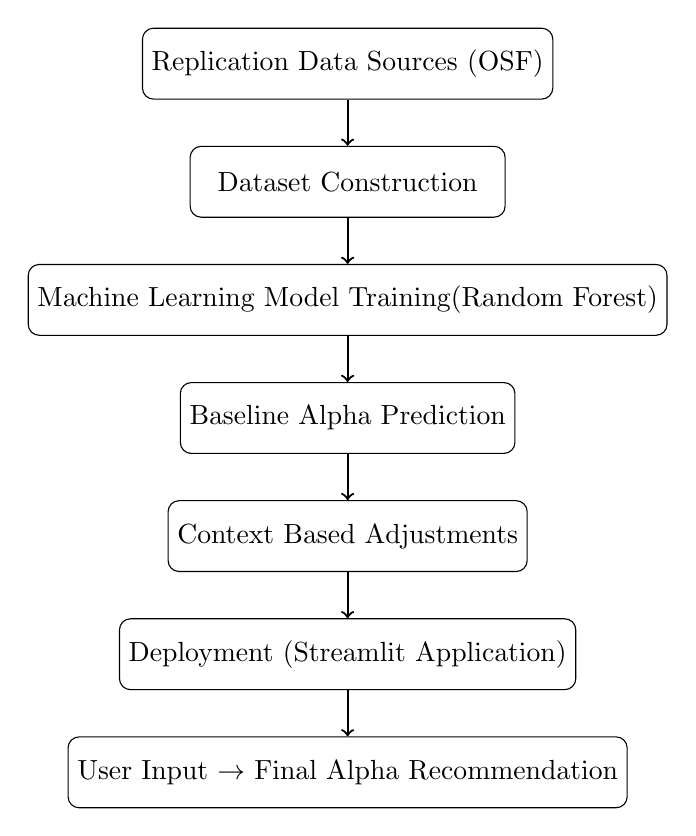
\begin{tikzpicture}[
		node distance=1.5cm,
		every node/.style={draw, rectangle, rounded corners, align=center, minimum width=4cm, minimum height=0.9cm},
		arrow/.style={->, thick}
		]
		
		\node (data) {Replication Data Sources (OSF)};
		\node (dataset) [below of=data] {Dataset Construction};
		\node (training) [below of=dataset] {Machine Learning Model Training(Random Forest)};
		\node (prediction) [below of=training] {Baseline Alpha Prediction};
		\node (adjustment) [below of=prediction] {Context Based Adjustments};
		\node (deployment) [below of=adjustment] {Deployment (Streamlit Application)};
		\node (output) [below of=deployment] {User Input $\rightarrow$ Final Alpha Recommendation};
		
		\draw[arrow] (data) -- (dataset);
		\draw[arrow] (dataset) -- (training);
		\draw[arrow] (training) -- (prediction);
		\draw[arrow] (prediction) -- (adjustment);
		\draw[arrow] (adjustment) -- (deployment);
		\draw[arrow] (deployment) -- (output);
		
	\end{tikzpicture}
	\caption{Machine Learning System Architecture}
	\label{fig:deployment_workflow}
\end{figure}
\section{Model Deployment}

The Alpha Recommendation System is deployed as an interactive application so that researchers can easily obtain an alpha recommendation without writing code. The deployed system allows users to enter study parameters and immediately receive a recommended significance level.

Figure \ref{fig:deployment_workflow} illustrates the overall workflow of the deployed system. The trained model developed in Chapter 4 is integrated into a Streamlit application. The following sections describe how users interact with the system to obtain an alpha recommendation.


\subsection{Purpose of Deployment}

The purpose of deployment is to make the developed model usable for researchers during the study planning stage. Instead of running Python scripts manually, users interact with the system through a simple interface for giving the application context inputs and getting displayed the results. 

\subsection{Choice of Deployment Tool}

The system is deployed using Streamlit, a Python framework for building interactive data applications. Streamlit allows a complete interface to be created directly from Python code without requiring additional web development technologies such as HTML or JavaScript\cite{streamlit-docs2024}.

This makes the system easy to run locally and accessible to users with limited programming experience.


\subsection{Loading the Trained Model}

After the machine learning model is trained during system development, it is saved as a serialized **`.pkl` file** using the Python *pickle* library. This file stores the trained model and its learned parameters.

During deployment, the Streamlit application loads the stored model when the application starts. This avoids retraining the model every time the system is used and allows predictions to be generated immediately.


The trained model is loaded using the following code:

\begin{lstlisting}[language=Python]
	import pickle
	
	with open("final_alpha_recommendation_system.pkl", "rb") as file:
	model = pickle.load(file)
\end{lstlisting}

Once loaded, the model is ready to generate predictions based on user inputs.


When the Streamlit application starts, this code loads the serialized model into memory. Once loaded, the model becomes available to the application and can immediately generate predictions based on user inputs. This approach improves efficiency because the computationally expensive training step does not need to be repeated each time the application is executed.

\section{User Interaction}

After the model is loaded, the application allows users to interact with the system through the Streamlit interface. Users provide the study parameters required for generating an alpha recommendation. The system then processes these inputs and returns the final result.


The interaction between the stored model, the Streamlit interface, and the prediction pipeline is illustrated in \ref{fig:prediction_workflow}

\subsection{User Input Interface}

The application provides a simple interface where users can enter the required study parameters. These include:
\begin{itemize}
	\item sample size
	\item expected effect size
	\item risk tolerance
	\item test type (one or two tailed)
	\item number of hypothesis tests
\end{itemize}

\begin{figure}[H]
	\centering
	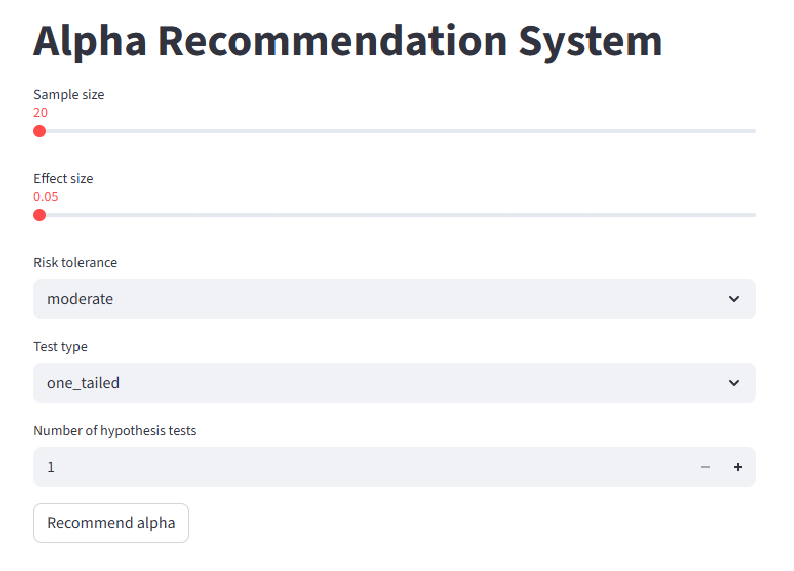
\includegraphics[width=0.7\textwidth]{Images/AlphaStreamlitBefore}
	\caption{Interface of the system before entering the values}
	\label{fig:BeforeInterface}
\end{figure}


Figure \ref{fig:BeforeInterface} shows the interface before the recommendation is generated.

The following code defines the input components of the Streamlit application:



\begin{lstlisting}[language=Python]
	
	import streamlit as st
	
	sample_size = st.number_input("Sample size", min_value=1)
	effect_size = st.number_input("Effect size", min_value=0.0)
	risk_level = st.selectbox("Risk tolerance",
	["very_strict", "strict", "neutral", 
	"lenient", "very_lenient"])
	tail_type = st.selectbox("Test type", 
	["two_tailed", "one_tailed"])
	num_tests = st.number_input("Number of hypothesis tests", 
	min_value=1)
	
\end{lstlisting}

These inputs are passed to the prediction pipeline to generate the recommendation.


\subsection{Generating the Alpha Recommendation}

Once the user enters the required parameters, the application generates the alpha recommendation in two steps.
\begin{itemize}
\item First, the trained machine learning model predicts a baseline alpha value using the input sample size and expected effect size.

\item Second, the system applies contextual adjustments based on the selected risk tolerance, test type, and number of hypothesis tests.
\end{itemize}

The implementation is shown below:

\begin{lstlisting}[language=Python]
	alpha_base = model.predict([[sample_size, effect_size]])[0]
	
	alpha_final = adjust_for_risk(alpha_base, risk_level)
	alpha_final = adjust_for_tail(alpha_final, tail_type)
	alpha_final = adjust_for_multiple_tests(alpha_final, num_tests)
	
	alpha_final = max(0.001, min(alpha_final, 0.15))
\end{lstlisting}

\begin{figure}[h]
	\centering
	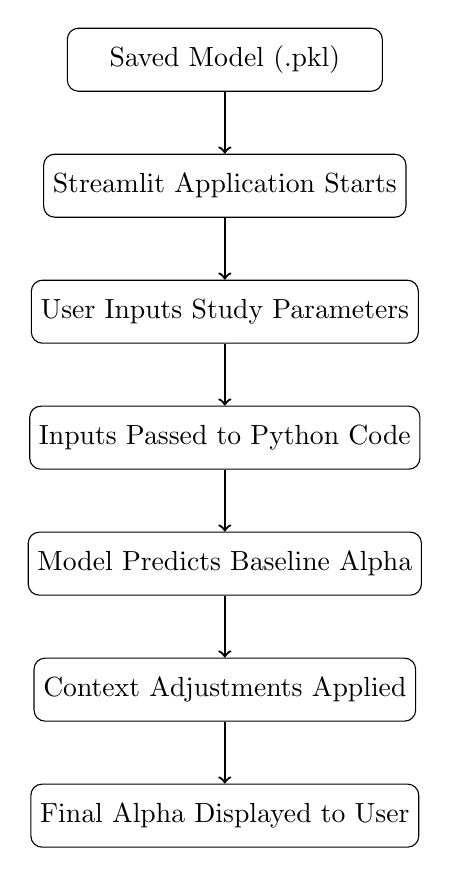
\begin{tikzpicture}[
		node distance=1.6cm,
		every node/.style={draw, rectangle, rounded corners, align=center, minimum width=4cm, minimum height=0.8cm},
		arrow/.style={->, thick}
		]
		
		\node (model) {Saved Model (.pkl)};
		\node (start) [below of=model] {Streamlit Application Starts};
		\node (input) [below of=start] {User Inputs Study Parameters};
		\node (code) [below of=input] {Inputs Passed to Python Code};
		\node (predict) [below of=code] {Model Predicts Baseline Alpha};
		\node (adjust) [below of=predict] {Context Adjustments Applied};
		\node (output) [below of=adjust] {Final Alpha Displayed to User};
		
		\draw[arrow] (model) -- (start);
		\draw[arrow] (start) -- (input);
		\draw[arrow] (input) -- (code);
		\draw[arrow] (code) -- (predict);
		\draw[arrow] (predict) -- (adjust);
		\draw[arrow] (adjust) -- (output);
		
	\end{tikzpicture}
	\caption{Prediction workflow of the deployed System}
	\label{fig:prediction_workflow}
\end{figure}

The overall prediction workflow of the deployed system is illustrated in Figure \ref{fig:prediction_workflow}.

\subsection{Displaying Results to the User}

After the calculations are completed, the final recommended alpha value is displayed clearly in the interface.

Figure \ref{fig:AfterInterface} shows the interface after the user has entered the inputs and generated the recommendation. The highlighted output box presents the final context-adjusted alpha value.
\begin{figure}[H]
	\centering
	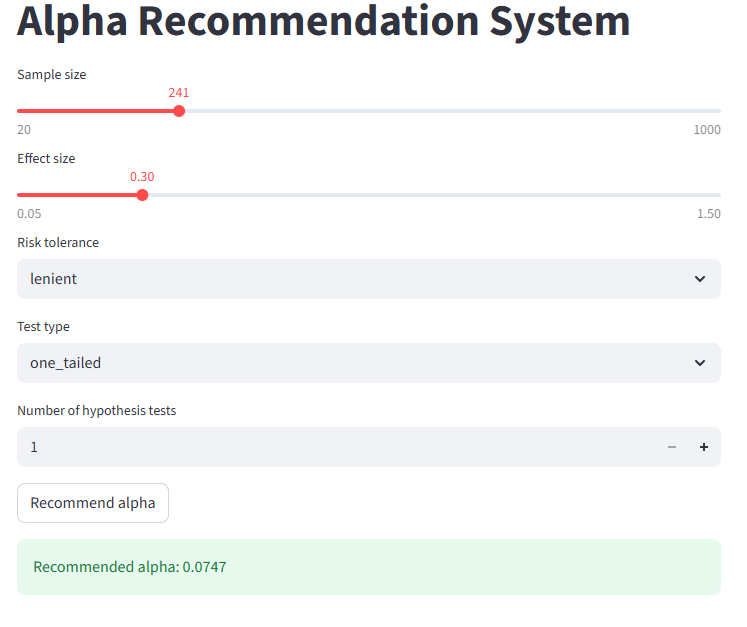
\includegraphics[width=0.7\textwidth]{Images/StreamlitAlphaAfter}
	\caption{Interface of the system after entering the values}
	\label{fig:AfterInterface}
\end{figure}

In the example shown, a study with a sample size of 241, an expected effect size of 0.30, a lenient risk tolerance, a one-tailed test, and one hypothesis test results in a recommended alpha value of 0.0747. This value is generated through the predictive model and subsequent contextual adjustments.

After the final alpha value has been computed, the application must communicate the result to the user through the interface. The following code implements the output component of the deployed application. It retrieves the final alpha recommendation generated by the prediction pipeline and displays it in the Streamlit interface. This step completes the interaction cycle by presenting the result of the model prediction and contextual adjustments in a clear and accessible format for the user.

The display is implemented as follows:

\begin{lstlisting}[language=Python]
	st.write("Recommended significance level (alpha):")
	st.success(round(alpha_final, 4))
\end{lstlisting}

This allows the user to immediately view the recommended alpha value based on the provided study parameters.

\subsection{Running the Application}

To allow other researchers to use the developed system, the implementation code will be made available through a public GitHub repository. This allows users to download the application and run it on their own computer.

To execute the system, the user first downloads or clones the repository from GitHub. The repository contains the trained model file, the application code, and the required dependencies.

After downloading the project, the required Python libraries must be installed. These include libraries such as streamlit, pandas, numpy, and scikit-learn.

Once the dependencies are installed, the application can be started using the following command in the project directory:

\begin{verbatim}
	streamlit run app.py
\end{verbatim}

When the application starts, Streamlit automatically opens the interface in a web browser. The user can then enter the required study parameters, such as sample size, effect size, risk tolerance, test type, and number of hypothesis tests.

After providing the inputs and clicking the recommendation button, the system generates and displays the recommended alpha value.

This setup allows the Alpha Recommendation System to be easily executed and reused by other researchers.

The source code for the system is available in the project repository \url{https://github.com/Abishek700/AlphaPredictionSystem}.

The GitHub repository link is provided in Appendix A.

\section{Summary}

In summary, the Alpha Recommendation System is deployed as a lightweight Streamlit application that enables user interaction in a straightforward and transparent manner. The trained model is loaded once, inputs are collected through a structured interface, and alpha recommendations are generated through a clearly defined two-stage process. This deployment approach allows the system to function as a practical tool for study planning while maintaining clarity and interpretability.